
\chapter{WebRTC}

\section{Co to jest, z czego się składa?}

Beniz \cite{hpbn} eniz

WebRTC jest projektem zapewniającym przeglądarkom możliwości komunikacji czasu rzeczywistego, dzięki czemu możliwe jest
budowanie komunikatorów internetowych w całości w obrębie zapewnianego przez przeglądarkę javascriptowego API. Aby
funkcjonalność ta była możliwa do zrealizowania, niezbędne było użycie wielu protokołów sieciowych, które pokazano
na rysunku \ref{fig:webrtc_stack}.

\begin{figure}[htbp]
	\centering
	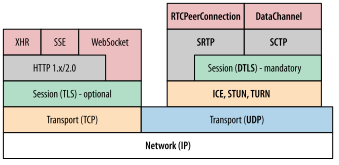
\includegraphics{img/webrtc-stack_hpbn}
	\caption{Stos protokołów w WebRTC - wzięty z HPBN - do zmiany}
	\label{fig:webrtc_stack}
\end{figure}

\section{Sygnalizacja nawiązania połączenia}


\section{Interactive Connectivity Establishment (ICE)}

\section{Opis API WebRTC}

